% Preamble
% ---
\documentclass{article}

% Packages
% ---
\usepackage{amsmath} % Advanced math typesetting
\usepackage[utf8]{inputenc} % Unicode support (Umlauts etc.)
\usepackage{hyperref} % Add a link to your document
\usepackage{graphicx} % Add pictures to your document
\usepackage{listings} % Source code formatting and highlighting
\usepackage{framed} % Source code formatting and highlighting
\usepackage{appendix} % Source code formatting and highlighting
\usepackage{csquotes} % Pretty quotes
\usepackage{xcolor}
\usepackage{pagecolor}
\usepackage[letterpaper, portrait, margin=1.5in]{geometry}

\graphicspath{ {images/} }

\definecolor{limegreen}{HTML}{bbe963}


\title {XYO Cryptoeconomics}

\author{
    Aaron Malone \thanks{Commonly known as "PizzaMind"}\\
    \and
    Arie Trouw\\
    \and    
    Bryce Paul\\
    \and
    Erik Saberski\\
    \and
    Nate Brune \thanks{Commonly known as "Machete"}\\
    \and
    Scott Scheper\\
}

\date{May 2019 \\ Version 2.0.0 (Dracarys)\\ \texttt{STATUS: DRAFT}}




\begin{document}

\pagecolor{limegreen}

\maketitle

\begin{center}
\line(1,0){50}
\end{center}

\begin{abstract}
This document outlines the XYO Cryptoeconomic plan and sets forth an intriguing idea of tethering a cryptoasset to \textit{data flow}. First, we provide supporting background knowledge of XYO's Cryptoeconomics. Then we lay forth the plan to grow XYO's network through finalizing the allocation of the GAMMA XYO Token Pool. Finally, we lay forth an intriguing idea of tethering XYO to the amount of valuable \textit{data flow} in the network.
\end{abstract}

\section{Background}
The XYO Network is an open cryptonetwork of IoT devices running an protocol that provides useful geospatial data to the world. The incentive mechanism built into the protocol is a type of cryptoasset called a \textit{protocol token}. This protocol token is built into the XYO Network and is named ``XYO'' (also referred to as ``XYO Token'' and ``XYO Cryptoasset'').

\subsection{The Cryptoeconomic Reserve}
We conducted the XYO Token Main Sale from March 20, 2018 - May 20, 2018. A total of 14,198,847,000 XYO was distributed. The rest of the XYO Tokens were burned.\\
\\During the XYO Token Sale, a pool of XYO was created, called “The Cryptoeconomic Reserve”.

\begin{displayquote}\textit{``The goal of the Cryptoeconomic Reserve is to provide incentives to network participants in order to jump-start the foundation of the network.''} \cite{crypto-reserve}
\end{displayquote}

The Cryptoeconomic Reserve is intended for the following items:

\begin{enumerate}
  \item Incentivizing blockchain developers to create dApps that interact with XYO.
  \item Incentivizing Geominers (Operators of the four types of XYO Nodes: Sentinels, Bridges, Archivists and Diviners)
  \item Incentivizing XYO Token usefulness and network activity
  \item Facilitating decentralization amongst nodes
  \item Incentivizing artificial intelligence in edge nodes (Sentinels and Bridges)
\end{enumerate}


There is a total of 2,871,068,696.85 XYO in the Cryptoeconomic Reserve (~2.8 Billion).

\subsection{GAMMA Token Pool}

\begin{itemize}
	\item 5 billion XYO Tokens were allocated to a pool to be sold to the public. This enabled a decentralized XYO Token Pool (where the public owns and controls the majority of XYO).
	\item  659,855,226.56 XYO was sold during the GAMMA Sale.
	\item  The GAMMA Sale ended on November 30, 2018. The left-over amount of XYO is 4,340,144,773.44 in the GAMMA Token Pool.
\end{itemize}


\subsection{Founding HODL'er Registry (FHR)}

\begin{itemize}
	\item The FHR is comprised of those who \texttt{purchased} directly from the XYO Network core team from January 6, 2018 to November 30, 2018. See XIP-1.\cite{xip-1}.
	\item  The FHR List does \texttt{NOT} include any of the following participants: employees, partners, sponsors or individuals who received XYO without purchasing it. Only those who participated in the XYO Token Sales by \textit{purchasing} XYO are included in the FHR.
	\item One may view the FHR here: \textit{https://matrix.xyo.network/fhr}.
\end{itemize}

Our XYO Founding HODL'ers form a special part of XYO's story and they're a big reason for our success! They shall not be forgotten.

\section{The Plan}

\subsection{XYO Token Distribution to FHR}

First, we will be distributing XYO to those in the Founding HODL'er Registry as follows:

\begin{enumerate}
\item 340,144,773.44 XYO will be distributed to those on the FHR. 
\item When distributed, the XYO can be withdrawn by the FHR Wallet Address.
\item The XYO will be distributed on a pro-rata basis, meaning the amount of XYO you receive is based on the amount of XYO you originally purchased \textit{and still hold}.
\item The XYO of The FHR will put in a separate wallet address and will be distributed to the FHR so that the community can monitor it.
\end{enumerate}

\subsection{Timeline of FHR Distribution}

On or before December 1, 2019, the XYO will begin being distributed to the FHR members on a regular basis (i.e. monthly) for a period of 5 years.
\subsubsection{FHR Members}

If you are an XYO Founding HODL'er:

\begin{enumerate}
  \item The ``H'' in FHR stands for \textit{HODL} (crypto speak for ``hold'').
  \item Thus, it is recommended that you hold the entire amount of XYO you've purchased in your FHR Wallet.
  \item If you are unable to do this because you've transferred your XYO to another wallet (in cold storage for instance), that is OK \textit{as long as that cold storage wallet has at least the amount of XYO you purchased using the FHR Wallet}.
  \item We will be building a tool in the Matrix enabling you to white list wallet addresses that belong to you. \textit{In the meantime, we recommend you move your XYO back to your XYO FHR Wallet Address}.
  \item Holding more XYO in your FHR Wallet Address than you purchased is also recommended. This will be factored into XYO reward multiples and Geodapp rewards. For example, if you purchased 100,000 XYO during the XYO Token Sale or in GAMMA, and you've since bought 50,000 more XYO), you may receive higher reward multiples if you hold 150,000 XYO in your FHR Wallet.
  \item \textit{Because of this, we recommend you hold all of your XYO in your FHR Wallet (Reminder: Please keep your private keys secure)}.
\end{enumerate}


\subsection{XYO Token Distribution to Cryptoeconomic Reserve}

With the XYO Mainnet launched and staking live, we will begin focusing on growing the XYO Network by using the Cryptoeconomic Reserve to acquire and train new customers (XYO Node Operators, aka "Geominers").\\

One of the ways we will deploy this is through selling XYO Cryptoeconomic Packages.\\

The remaining 4,000,000,000 in XYO from the GAMMA Token Pool will be allocated to the Cryptoeconomic Reserve. We will begin deploying this via the XYO Cryptoeconomic Packages covered next.

\subsection{XYO Cryptoeconomic Packages}

Here is a sample of the products that the XYO Cryptoeconomic Packages will include:

\begin{enumerate}
  \item XYO
  \item XYO Geominers (SentinelX's, XYO Bridges, Geomining Kits)
  \item Geohacker Summit Ticket(s) - Hosted Monthly in San Diego, CA (Hands-on training and teaching one how to set up and operate XYO nodes)
  \item Dedicated VIP Concierge Phone Support and Training
  \item There will be additional items, as well
\end{enumerate}

\subsubsection{XYO Sold via Cryptoeconomic Packages Includes Network Staking}

Every XYO Sold in Cryptoeconomic Packages use \textit{Network Staking}.\\

This means, every XYO sold through the Cryptoeconomic Reserve has a staking period of 180 days minimum.\\

In the XYO Network, there are two types of staking, which we will cover next.

\subsection{XYO Staking: The Two Types}

\subsubsection{Network Staking}

The first type of staking is called \textit{Network Staking}. This comprises the act of staking your XYO for use in the XYO Network (between or amongst any nodes in the XYO Network).\\

Once you execute a Network Stake, you lock your XYO in the XYO Network ecosystem and can transfer the XYO between your own XYO nodes at any time. However, you cannot withdraw your XYO until the Network Stake Period has ended.\\

The Network Stake Period can be selected when initially staking your XYO tokens. This longer this the Network Stake Period, the greater it's compounding interest will be. The amount of stake you have determines the proportion of the mining pool you obtain daily.\\



Below is the comparison of the value of stakes for two examples of an initial 1000 XYO staked for 10 years. The blue line represents a staking period of 1 year, repeatedly staked 10 times, thus allowing the owner to redeem their XYO 10 different times. The green line represents a single Network Stake Period of 10 years, not allowing the owner to redeem it until the end of the 10 years. It is clear that the longer one initially commits to the length of their stake, the more valuable it will become.

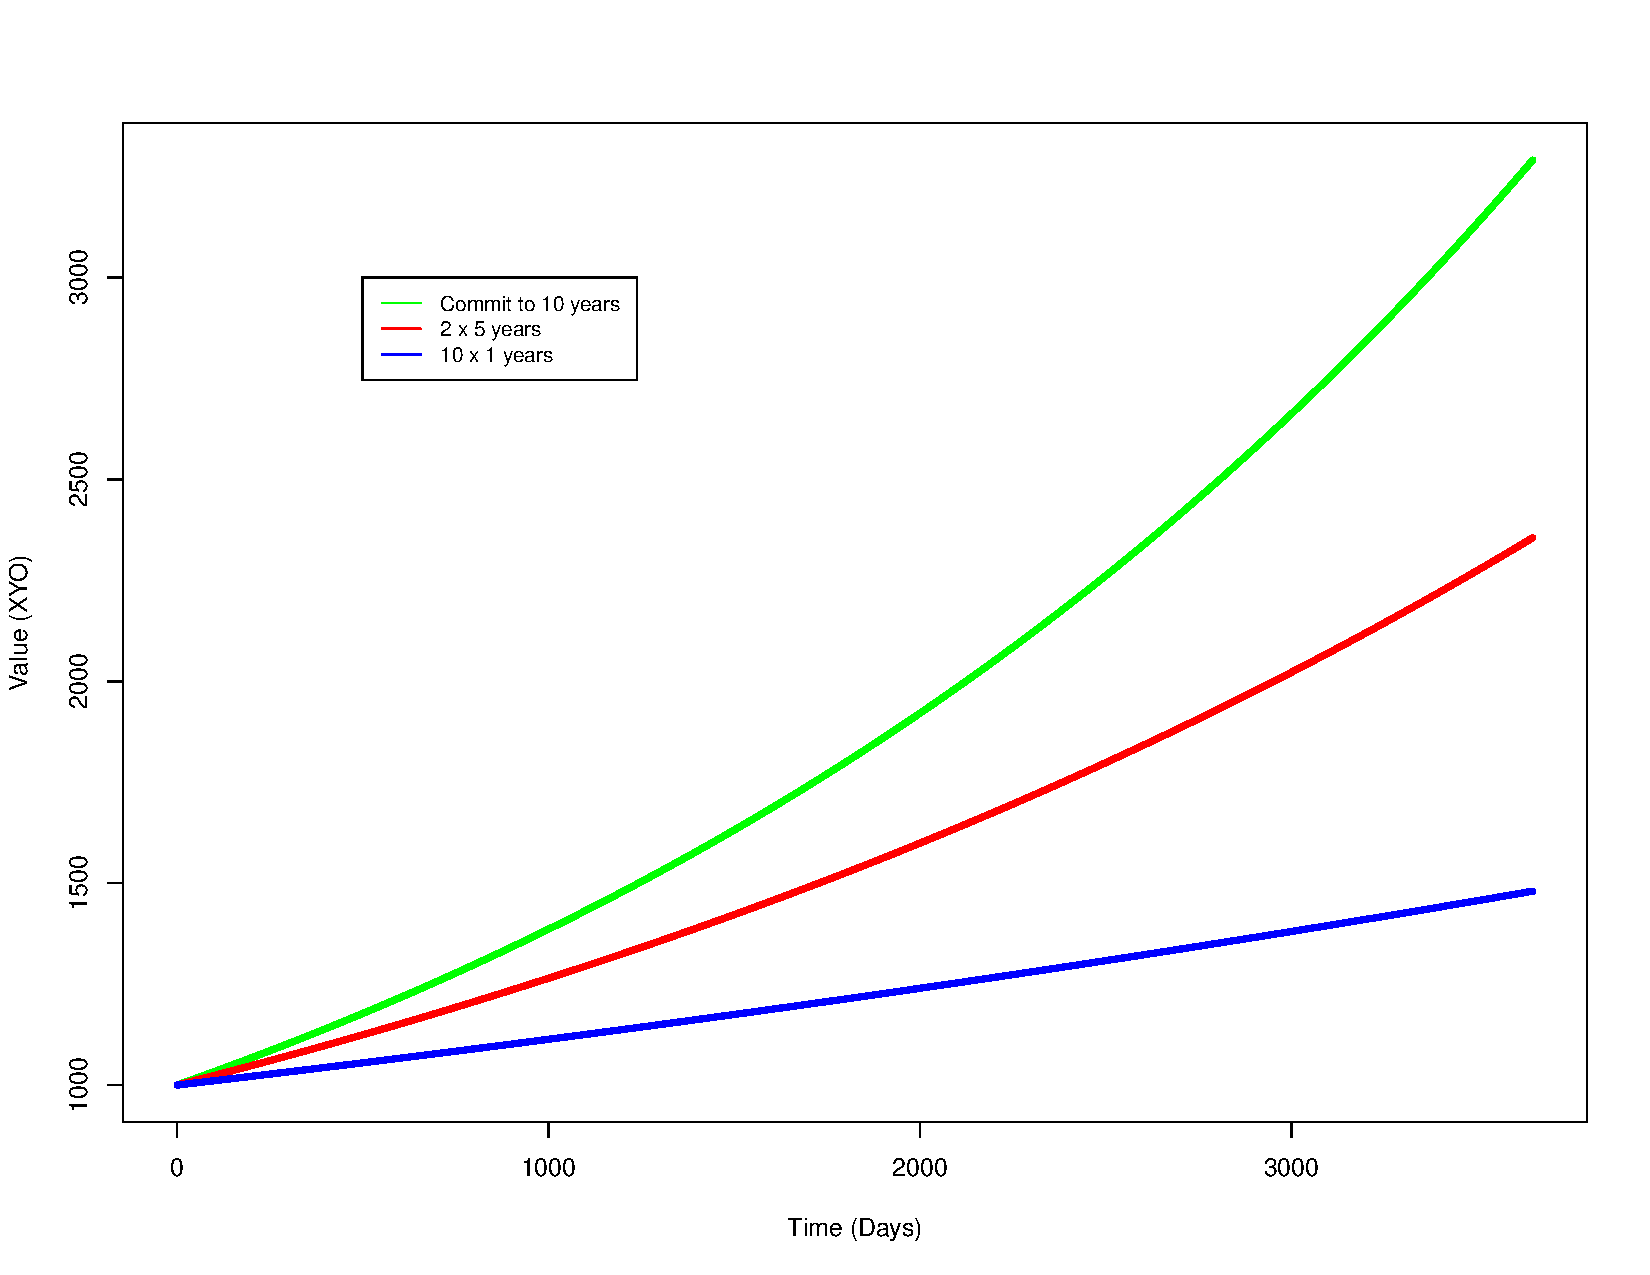
\includegraphics[width=\textwidth]{StakingAlgorithm.pdf}
\\\\

This is generated from the equation below:
\begin{align}
    Value &= stake(1+r)^{t/365}\\
    r &= \frac{\sqrt{N}}{\alpha}
\end{align}
where $t$ is the amount of time the stake has been locked in, $N$ is the Network Staking Period, and $\alpha$ is an adjustable scaling constant ($\alpha = 25$ in the plot above).

\subsubsection{Node Staking}

The second type of staking is called \textit{Node Staking}. This staking is conducted when you stake one of the four types of XYO Nodes (Sentinel, Bridge, Archivist, Diviner).\\ 

Node-staking has a five-day unfreezing period. Meaning when you withdraw your XYO into your Ethereum ERC-20 Wallet, it takes five-days before it’s withdrawn from the network.

\subsubsection{Data Flow Index}

The XYO Cryptoasset is used for rewarding positive participation in the XYO Network. The value of the network does not necessarily correlate directly to the value of the XYO Cryptoasset; rather, the value of the network is a measure of the value of the data it holds. Both the XYO Cryptoasset and the Data Flow Index are both driven by the same causal variables, which may result in correlation to one another. \\\\

Calculating the value of data is not necessarily straightforward. Listed below are reasons why this is. [1]:

\begin{enumerate}
  \item Data is (infinitely) shareable without any loss of value.
  \item Its value increases with use (unlike many typical assets).
  \item Data is perishable; the longer you keep it, the less use it is.
  \item The value of data increases with accuracy.
  \item Value increases when data is utilized with other data and/or information.
  \item More is not necessarily better.
  \item The amount of data cannot be depleted; rather, the more you use it, the more you have (Glazer, 1993).
\end{enumerate}
With this in mind, we determined a ``Data Flow Index''. The Data Flow Index that represents the value of the XYO Network and the data that flows through it. This Data Flow Index is calculated as:

\begin{equation}
Data Flow Index = \frac{\sum_{0}^{N}\sum_{0}^{n}S_dU}{R}
\end{equation}

where $\sum^{n}_{0}{S_d}$ is the sum of the stakes of all of the devices that have a piece of data in their origin chain, $U$ is the number of times that a piece of data was used to answer a query, $N$ is the number of pieces of data in the XYO Network, and $R$ is the amount of XYO paid out. This value can be calculated per any unit time (e.g. per day) to generate a time series of Data Flow Index. \\
This equation makes Data Flow Index a dimensionless quantity, with units of XYO (staked) in the numerator, and XYO (paid) in the denominator. Intuitively, as the number of nodes in the network increases, and as more devices are staked $S_d$ will increase. As the number of queries increases, both $U$ and $R$ will increase. However, with positive network growth, the Data Flow Index will exponentially grow since the increase in the numerator will be exponential compared to the increase in rewards paid out.\\
Since nodes are paid out in proportion to their stake, as the network grows the amount of XYO paid out to each device will, on average, decrease. This is simply because there will be more nodes on the network, but the same amount (or less) XYO circulating. However, the value behaves inversely to the payout; although devices are being paid less per amount of stake they have over time, the value of XYO per stake will be exponentially increasing. This can be thought of as our network contains and utilizes more data, the XYO Cryptoasset is backed by more value (i.e. the value of the network).

\subsection{Staking and Data Flow Index Q\&A}

\subsubsection{Why is it called Data Flow Index and not Data Value Index?}

The term \textit{Data Flow} encompasses the collection, storing, transfer, processing and paying for data. 

The reason we prefer the term Data Flow is because we as humans overvalue our capacity to determine good data is. The one exception is \textit{redundant data}. Redundant data is not good or valuable. However, as a species, homo sapiens are not the ones that should determine the value of non-redundant data \cite{homo-deus-narrative}. 

Therefore, we should focus on systems that increase data collection, storage, transfer and processing. In other words, systems that increase Data Flow. 

That’s essentially the flow of data. 

\subsubsection{Can I stake devices even if they are not mine?}
Yes! It is highly encouraged that you stake devices that you believe will earn more rewards. However, keep in mind that the more people that stake a device, the more the pot of rewards will be split. So it may not be in your best interest to stake only the most popular devices since their rewards will be heavily split. Rather, you may want to stake devices you specifically know will house your data.

\subsubsection{Is everyone staking the same devices?}
Theoretically, everyone could stake the same devices. But, as mentioned in the answer above, it would not be in peoples' best interest to all stake the same device. But theoretically, yes, everyone that stakes a specific archivist, for example, is waging for the validity of that archivist.

Using this model, we plan to track the Data Flow Index on a weekly basis. We intend to monitor it closely and adjust the model as needed.

\subsection{Price of XYO From Cryptoeconomic Reserve}

\begin{itemize}
  \item The price of the XYO will be sold at market price. Because the XYO sold from the Cryptoeconomic Reserve will be burned on a 1:1 basis (see below), the price of the XYO will be sold at the market price at time of purchase.
  \item Pricing will be adjusted according to the network growth, the XYO Data Flow Index, as well as other factors which we will determine over time.
  \item When we determine the Data Flow Index is mature, we plan to create an Ethereum smart contract, which tracks the Data Flow Index and tethers the price of XYO distributed through the Cryptoeconomic Reserve to the Data Flow Index.
\end{itemize}

\subsubsection{Dracarys: XYO Token Burn on 1:1 Basis}

\begin{itemize}
	\item For every 1 XYO Sold, there will be 1 XYO from the Cryptoeconomic reserve which will be burned. This will proceed until 50\% of the Cryptoeconomic Reserve is burned (up to 3,250,034,273.430 XYO).
	\item Burning will take place either monthly or quarterly depending on how much we can streamline the process. We will know after our first XYO Token Burn. We're targeting the first burn to be end of June 2019 or first week of July 2019. We will put out a news release and update before the first burn.
	\item The XYO burned will be sent into an Ethereum Wallet Address (the "Dracarys Address"). We'll provide this address once created so that the community can monitor it and celebrate the burn event when it's sent to a smart contract and burned.
\end{itemize}  

\subsubsection{Repurchasing XYO}
\begin{itemize}
	\item Each week between 5 and 15\% of XYO Product Packages sold from the Cryptoeconomic Reserve will be used to purchase XYO on exchanges.
	\item We'll be providing the Ethereum Wallet Address of the pool of ETH, which will be used to purchase XYO on exchanges so that the community can monitor this. 
	\item The ETH will be deployed and purchased on a regular basis (meaning daily).
\end{itemize}

\begin{center}
\line(1,0){50}
\end{center}

\begin{thebibliography}{9}

\bibitem{crypto-reserve}
XYO Network
\\\texttt{https://xyo.network}.
March 2018.

\bibitem{xip-1}
XYO Improvement Protocol \#1
\textit{XYO Geohacker Forum}.
\\\texttt{https://geohacker.xyo.network/t/status-accepted-xip-1-founding-hodler-registry-fhr/927/104}.
March 2018.

\bibitem{homo-deus-narrative} 
Harari, Yuval Noah
\textit{Homo Deus (p. 296)}. 
Harper.


\end{thebibliography}

%*******************************
%**** End Glossary Section *****
%*******************************

\end{document}
